

\begin{frame}{\ft{\AtR{} Applications as Data Collection Instruments}}
\section{Research Slide 3}
%\doubleFrame{In medicine and social science, \q{data collection instruments} 
%(DCIs) refer to surveys, questionnaires, and other tools to get human feedback.}

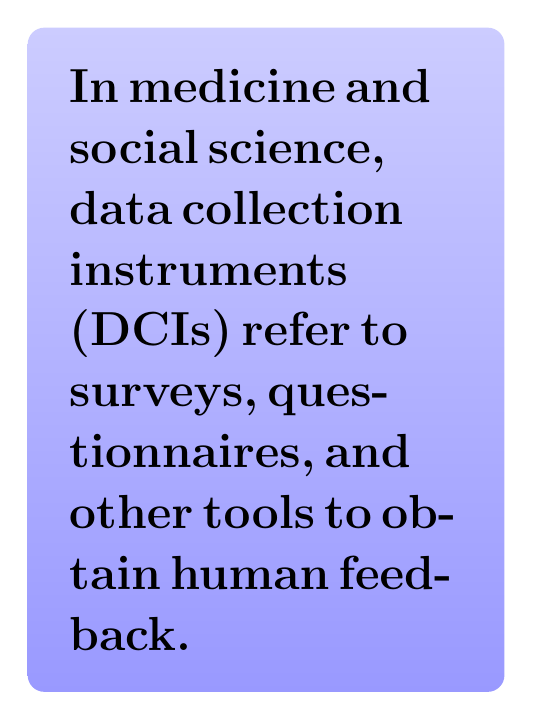
\begin{tikzpicture}
\nodeincludegraphicsTRRS{1}{0cm}{0cm}{0cm}{0cm}{pics/Res-2a.jpeg}

 \node [anchor=west,inner sep=15, text width=5cm,top color=blue!20,
 bottom color=blue!40,
 rounded corners=6pt%,
 %blur shadow={shadow blur steps=2}
 ]
  (longnote) at (15.5,8) {\baselineskip=22pt%  %{\color{rb!85!red}{
  {\LARGE \textbf{In medicine and \makebox{social} science, \q{data collection \makebox{instruments}} 
(DCIs) refer to surveys, questionnaires, 
and other tools to obtain human feedback.}}\par};

\end{tikzpicture}


\end{frame}

